% ---------------------------------------------------------------------------
% Neudata Consulting Ltd — report template, STYLE 2 (Overleaf ready)
% Matches the Neudata PowerPoint template: white cover, teal headings,
% "Neudata | #ClearDataClearImpact" footer. For the Quarto look see main.tex.
% Other class options: report | proposal | note, draft, nocover
% ---------------------------------------------------------------------------
\documentclass[style2, report]{neudata}

\usepackage[style=authoryear, backend=biber, maxcitenames=2]{biblatex}
\addbibresource{references.bib}

\title{Report title}
\subtitle{Short descriptive subtitle}
\author{Analyst Name}
\affiliation{Neudata Consulting Ltd}
\client{Client organisation}
\reference{NDC-2026-000}
\confidentiality{Confidential}
% \version{1.0}
% \date{29-04-2026}          % defaults to today, DD-MM-YYYY
\abstract{One-paragraph executive summary: the question, the data, the approach and the
  headline finding. Keep it readable by a non-technical decision-maker.}

\begin{document}

\maketitle
\tableofcontents
\clearpage

\section{Introduction}

Describe the background, the client's objective and the questions this report answers.

\begin{keyfindings}
  \begin{itemize}
    \item Finding one, stated plainly with its size and uncertainty.
    \item Finding two.
    \item Recommendation or implication for the client.
  \end{itemize}
\end{keyfindings}

\section{Data and methods}

Summarise the data sources, inclusion criteria, variables and statistical methods. Refer to the
statistical analysis plan for full detail \parencite{lumley2004}.

\section{Results}

\subsection{Descriptive summary}
Table~\ref{tab:summary} summarises the example data.

\begin{table}[ht]
  \centering
  \caption{Mean tooth length by supplement and dose (example data).}
  \label{tab:summary}
  \begin{tabular}{lrr}
    \toprule
    \neudataheader \neudatath{Supplement} & \neudatath{Dose (mg/day)} & \neudatath{Mean length} \\
    \midrule
    OJ & 0.5 & 13.2 \\
    VC & 0.5 &  8.0 \\
    OJ & 1.0 & 22.7 \\
    VC & 1.0 & 16.8 \\
    OJ & 2.0 & 26.1 \\
    VC & 2.0 & 26.1 \\
    \bottomrule
  \end{tabular}
\end{table}

\subsection{Main analysis}
Figure~\ref{fig:main} shows the relationship using the Neudata palette.

\begin{figure}[ht]
  \centering
  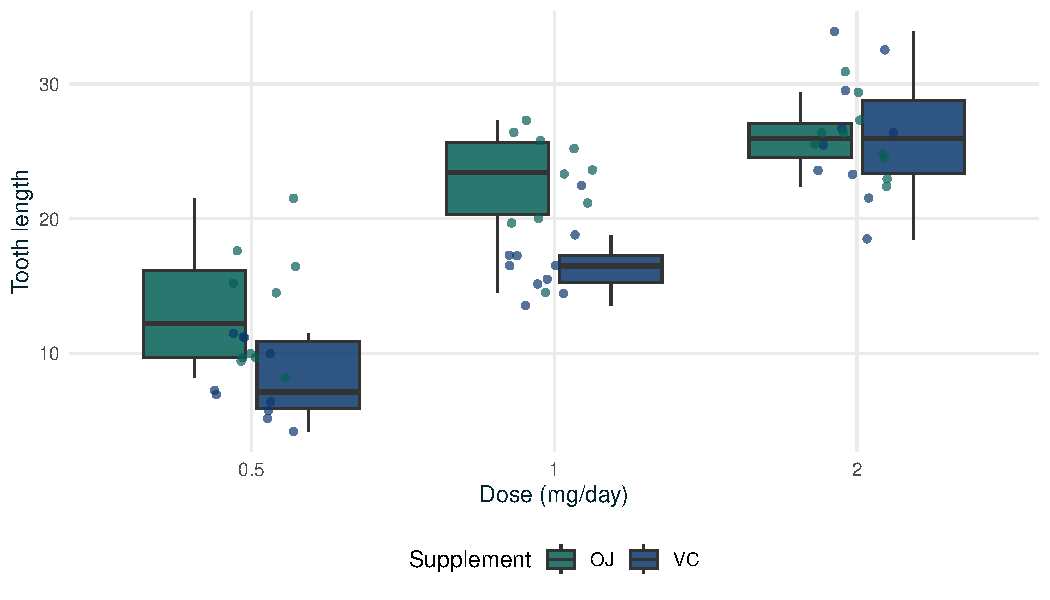
\includegraphics[width=0.9\textwidth]{figures/example-figure.pdf}
  \caption{Tooth length by dose and supplement (example data).}
  \label{fig:main}
\end{figure}

\section{Discussion}

Interpret the results, note limitations and set out recommendations.

\begin{neudatanote}[Reproducibility]
  This report was generated from code. Software versions are listed in the appendix.
\end{neudatanote}

\printbibliography[heading=bibnumbered]

\appendix
\section{Appendix}

Supplementary tables, code listings and software versions.

\neudatacopyrightpage

\end{document}
